\section{Overview}
\label{sec:overview}

\myparagraph{Knowledge-based policies and beliefs}  User Bob would
like to enforce a knowledge-based policy on his data so that
advertisers do not learn too much about him.  Suppose Bob considers
his birthday of September 27, 1980 to be relatively private; variable
$\var{bday}$ stores the calendar day (a number between 0 and 364,
which for Bob would be 270) and
$\var{byear}$ stores the birth year (which would be 1980).  To
$\var{bday}$ he assigns a \emph{knowledge threshold} $t_{\var{d}} =
0.2$ stating that he does not want an advertiser to have better than a
20\% likelihood of guessing his birth day.  To the pair
$(\var{bday},\var{byear})$ he assigns a threshold $t_{\var{dy}} =
0.05$, meaning he does not want an advertiser to be able to guess the
combination of birth day \emph{and} year together with better than a
5\% likelihood.

Bob runs an agent program to answer queries about his data on his
behalf.  This agent models an estimated \emph{belief} of queriers as a
probability distribution $\delta$, which is conceptually a map from
secret states to positive real numbers representing probabilities (in
range $[0,1]$).  Bob's secret state is the pair $(\var{bday}\! =\!
270,\var{byear}\! =\! 1980)$.  The agent represents a distribution as a
set of probabilistic polyhedra.  For now, we can think of a
probabilistic polyhedron as a standard convex polyhedron $\getpoly{}$
with a probability mass $m$, where the probability of each integer
point contained in $\getpoly{}$ is $m / \psize{\getpoly{}}$, where
$\psize{\getpoly{}}$ is the number of integer points contained in the
polyhedron $\getpoly{}$.  Shortly we present a more involved
representation.

Initially, the agent might model an advertiser $X$'s belief using the
following rectangular polyhedron $\getpoly{}$, where each point
contained in it is considered equally likely ($m = 1$):
$$
\begin{array}{l}
\getpoly{} = 0 \leq \var{bday} < 365,\; 1956 \leq \var{byear} < 1993
\end{array}
$$

\myparagraph{Enforcing knowledge-based policies safely} Suppose $X$
wants to identify users whose birthday falls within the next week, to
promote a special offer.  $X$ sends Bob's agent the following program.
\begin{example} 
\label{ex:bday}
\begin{displaymath}
\begin{array}{l}
\sassign{\var{today}}{260}; \\
\sifk\; {\var{bday} \geq today \wedge \var{bday} < (today+7)}\;\sthenk \\
\quad \sassign{\var{output}}{\strue};\\
\end{array}
\end{displaymath}
This program refers to Bob's secret variable $\var{bday}$, and also
uses non-secret variables $\var{today}$, which represents the current
day and is here set to be 260, and $\var{output}$, which is set to
$\strue$ if the user's birthday is within the next seven days (we
assume $\var{output}$ is initially $\sfalse$).
\end{example}

The agent must decide whether returning the result of
running this program will potentially increase $X$'s knowledge
about Bob's data above the prescribed threshold.  We explain how it
makes this determination shortly, but for the present we can see that
answering the query is safe: the returned $\var{output}$ variable will
be $\sfalse$ which essentially teaches the querier that Bob's birthday
is not within the next week, which still leaves many possibilities.  As
such, the agent \emph{revises} his model of the querier's belief to be
the following \emph{pair} of rectangular polyhedra $\getpoly{1},
\getpoly{2}$, where again all points in each are equally likely
($m_1 \approx 0.726, m_2 \approx 0.274$):
$$
\begin{array}{l}
\getpoly{1} = 0 \leq \var{bday} < 260,\; 1956 \leq \var{byear} < 1993 \quad \\
\getpoly{2} = 267 \leq \var{bday} < 365,\; 1956 \leq \var{byear} <  1993 \quad \\
\end{array}
$$
Ignoring $\var{byear}$, there are 358 possible values for
$\var{bday}$ and each is equally likely. Thus the probability of any one is
$1 / 358 \approx 0.0028 \leq t_{\var{d}} = 0.2$.

\ifacita

Suppose the next day the same advertiser sends the same program to
Bob's user agent, but with $\var{today}$ set to 261.  At first glance
running this program seems OK.  The program will return $\sfalse$, and
the revised belief will be the same as above but with constraint
$\var{bday} \geq 267$ changed to $\var{bday} \geq 268$. There
is only a $1 / 357 \approx 0.0028$ chance to guess $\var{bday}$.

\else
Suppose the next day the same advertiser sends the same program to
Bob's user agent, but with $\var{today}$ set to 261.  Should the agent
run the program?  At first glance, doing so seems OK.  The program
will return $\sfalse$, and the revised belief will be the same as
above but with constraint $\var{bday} \geq 267$ changed to $\var{bday}
\geq 268$, meaning there is still only a $1 / 357 \approx 0.0028$ chance to
guess $\var{bday}$.
\fi

But suppose Bob's birth day was actually 267, rather than 270.  The
first query would have produced the same revised belief as before, but
since the second query would return $\strue$ (since $\var{bday}=267 <
(261 + 7)$), the querier can deduce Bob's birth day exactly:
$\var{bday} \geq 267$ (from the first query) and $\var{bday} < 268$
(from the second query) together imply that $\var{bday} = 267$!  But
the user agent is now stuck: it cannot simply refuse to answer the
query, because the querier knows that with $t_{\var{d}} = 0.2$ (or
indeed, any reasonable threshold) the only good reason to refuse is
when $\var{bday} = 267$.  As such, refusal essentially tells the
querier the answer.

The lesson is that the decision to refuse a query must not be based on
the effect of running the query on the actual secret, because then a
refusal could leak information.  In Section~\ref{sec:policy} we
propose that an agent should reject a program if there exists
\emph{any} possible secret that could cause a program answer to
increase querier knowledge above the threshold. As such we would
reject the second query regardless of whether $\var{bday} = 270$ or
$\var{bday} = 267$.

\myparagraph{Full probabilistic polyhedra} Now suppose, having run the first
query and rejected the second, the user agent receives the following
program from $X$.
\begin{example}
\label{ex:specyear}
\begin{displaymath}
\begin{array}{l}
\sassign{\var{age}}{2011 - \var{byear}}; \\
\sifk\; {\var{age} = 20 \vee ... \vee \var{age} = 60}\;\sthenk\;
\sassign{\var{output}}{\strue};\\
\spifnoelse{0.1}{\sassign{\var{output}}{\strue}};
\end{array}
\end{displaymath}
This program attempts to discover whether this year is a ``special''
year for the given user, who thus deserves a special offer.  The
program returns $\strue$ if either the user's age is (or will be) an
exact decade, or if the user wins the luck of the draw (one chance in
ten), as implemented by the probabilistic if statement.
\end{example}

\begin{figure}
\centering
\begin{tabular}{cc}
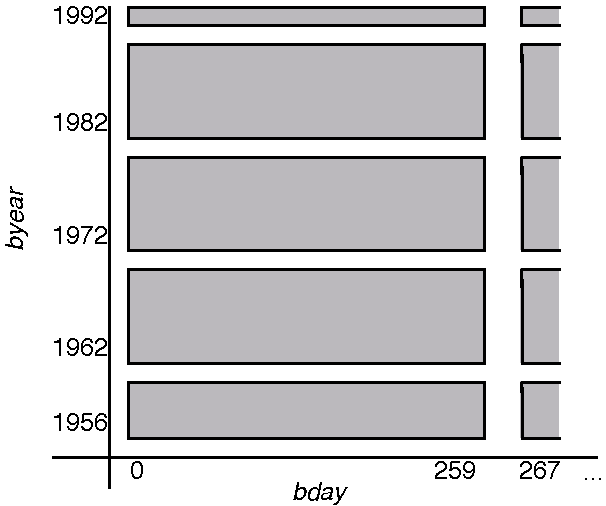
\includegraphics[width=4cm]{figures/bands1.pdf} &
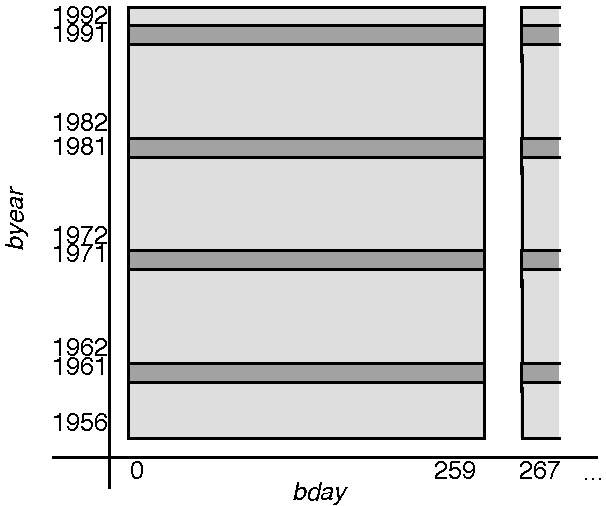
\includegraphics[width=4cm]{figures/bands2.pdf} \\
(a) $\var{output} = \sfalse$ & 
(b) $\var{output} = \strue$ \\
\end{tabular}
\caption{Example 2: most precise revised beliefs}
\label{fig:bands}
\end{figure}

\ifacita 
Running this program reveals nothing about $\var{bday}$, but
does reveal something about $\var{byear}$.  If $\var{output} =
\sfalse$ then the querier knows that $\var{byear} \not\in \{ 1991,
1981, 1971, 1961 \}$, but all other years are equally likely.  We
could represent this new knowledge, combined with the knowledge gained
from the first query, as in Figure~\ref{fig:bands}(a), where
each shaded box is a polyhedron containing equally likely points.  On
the other hand, if $\var{output} = \strue$ then either $\var{byear}
\in \{ 1991, 1981, 1971, 1961 \}$ or the user got lucky.  We represent
the querier's knowledge in this case as in Figure~\ref{fig:bands}(b).
Darker shading indicates higher probability; thus, all years are still
possible, though some are more likely than others.  With the
given threshold of $t_{\var{dy}} = 0.05$, the agent will permit the
query; when $\var{output} = \sfalse$, the likelihood of any point in
the shaded region is $1/11814$; when $\var{output} = \strue$, the
points in the dark bands are the most likely, with probability $
5/13067 $.  Since both outcomes are possible with Bob's $\var{byear} =
1980$, the revised belief will depend on the result of the
probabilistic if statement. 

\else
Running this program reveals
nothing about $\var{bday}$, but does reveal something about
$\var{byear}$.  In particular, if $\var{output} = \sfalse$ then the
querier knows that $\var{byear} \not\in \{ 1991, 1981, 1971, 1961 \}$,
but all other years are equally likely.  We could represent this new
knowledge, combined with the knowledge gained from the first query, as
shown in Figure~\ref{fig:bands}(a), where each shaded box is a
polyhedron containing equally likely points.  On the other hand, if
$\var{output} = \strue$ then either $\var{byear} \in \{ 1991, 1981,
1971, 1961 \}$ or the user got lucky.  We represent the querier's
knowledge in this case as in Figure~\ref{fig:bands}(b).  Darker
shading indicates higher probability; thus, all years are still
possible, though some are much more likely than others.  With the
given threshold of $t_{\var{dy}} = 0.05$, the agent will permit the
query; when $\var{output} = \sfalse$, the likelihood of any point in
the shaded region is $1/11814$; when $\var{output} = \strue$, the
points in the dark bands are the most likely, with probability $
5/13067 $.  Since both outcomes are possible with Bob's $\var{byear} =
1980$, the revised belief will depend on the result of the
probabilistic if statement.
\fi

This example illustrates a potential problem with the simple
representation of probabilistic polyhedra mentioned earlier: when
$\var{output} = \sfalse$ we will jump from using two probabilistic
polyhedra to ten, and when $\var{output} = \strue$ we jump to using
eighteen.  Allowing the number of polyhedra to grow without bound will
result in performance problems. To address this concern, we need a way
to abstract our belief representation to be more concise.
\ifacita
Our technical report~\cite{TR} 
\else
Section~\ref{sec:absinterp} 
\fi
shows how to represent a probabilistic
polyhedron $\pp{}$ as a seven-tuple, $(\getpoly{},\smin{}, \smax{}, \pmin{},
\pmax{}, \mmin{}, \mmax{})$ where $\smin{}$ and $ \smax{}$ are lower
and upper bounds on the number of points with non-zero probability
 in the polyhedron $\getpoly{}$ (called the \textit{support points} of $C$);
the quantities $\pmin{} $ and $ \pmax{} $ are lower and
upper bounds on the probability mass per support point; and $ \mmin{}
$ and $ \mmax{} $ give bounds on the total probability mass. Thus,
polyhedra modeled using the simpler representation $(\getpoly{},m)$
given earlier are equivalent to ones in the more involved
representation with $\mmax{} = \mmin{} = m$, $\pmax{} = \pmin{} = m /
\psize{\getpoly{}}$, and $\smax{} = \smin{} = \psize{\getpoly{}}$.

With this representation, we could choose to collapse the sets of
polyhedron given in Figure~\ref{fig:bands}.  For example, we could
represent Figure~\ref{fig:bands}(a) with two probabilistic polyhedra
$\pp{1}$ and $\pp{2}$ containing polyhedra $\getpoly{1}$ and
$\getpoly{2}$ defined above, respectively, essentially drawing a
box around the two groupings of smaller boxes in the figure.  The
other parameters for $\pp{1}$ would be as follows:
$$
\begin{array}{l}
\pmin{1} = \pmax{1} = 9/135050 \\
\smin{1} = \smax{1} = 8580 \\
\mmin{1} = \mmax{1} = 7722/13505 \\
\end{array}
$$
Notice that $\smin{1} = \smax{2} = 8580 < \psize{\getpoly{1}} = 9620$,
illustrating that the ``bounding box'' of the polyhedron covers more area
than is strictly necessary.  In this representation the probabilities may
not be normalized, which improves both performance and precision.  For this
example, $\pp{2}$ happens to have $\mmin{2} = \mmax{2} = 14553 / 67525 $ so we
can see $\mmax{1} + \mmax{2} = (53163 / 67525) \not= 1$.  

If we consider the representation of
Figure~\ref{fig:bands}(b) in a similar manner, using the same two polyhedra
$\getpoly{1}$ and $\getpoly{2}$, the other parameters for $\getpoly{1}$ are
as follows:
$$
\begin{array}{ll}
\pmin{1} = 1/135050 & \pmax{1} = 10/135050 \\
\smin{1} = 9620 & \smax{1} = 9620 \\
\mmin{1} = 26/185 & \mmax{1} = 26/185 \\
\end{array}
$$
In this case $\smin{1} = \smax{1} = \psize{\getpoly{1}}$, meaning that all
covered points are possible, but $\pmin{1} \not= \pmax{1}$ as some points
are more probable than others (i.e., those in the darker band).

The key property of probabilistic polyhedra, and a main technical
contribution of this paper, is that this abstraction can be used to make
sound security policy decisions.  To accept a query, we must check that, for
all possible outputs, the querier's revised, normalized belief of any of the
possible secrets is below the threshold $t$.  In checking whether the
revised beliefs in our example are acceptable, the agent will try to find
the maximum probability the querier could ascribe to a state, for each
possible output.  In the case $\var{output} = \strue$, the most probable
points are those in the dark bands, which each have probability mass
$10/135050 = \pmax{1}$ (the dark bands in $\pp{2}$ have the same
probability).
% But it is not enough to know
% this value.  We need to know how it compares to the probabilities of
% the other points.  That is, we have to \textit{normalize} the
% distribution before we can find the maximum probability of any point.
To find the maximum normalized probability of these points, we divide by the
minimum possible total mass, as given by the lower bounds in our
abstraction.  In our example, this results in $\pmax{1} / (\mmin{1} +
\mmin{2})$ $=$ $(10/135050) / (26/185 + 49/925) \approx 0.0004 \leq t_{\var{d}} = 0.05$.

As just shown, the bound on minimum total mass is needed in order to soundly
normalize distributions in our abstraction.  The maintenance of such lower
bounds on probability mass is a key component of our abstraction that is
missing from prior work.  Each of the components of a probabilistic
polyhedron play a role in producing the lower bound on total mass.  While
$\smin{1}, \smax{1}, \pmin{1},$ and $\mmax{1}$ do not play a role in making
the final policy decision, their existence allows us to more accurately
update belief during the query evaluation that precedes the final policy
check.  The choice of the number of probabilistic polyhedra to
use impacts both precision and performance, so choosing the right number is
a challenge.  
\ifacita
Section~\ref{sec:impl} shows that our implementation can
often answer these queries in seconds.
\else
For the examples given in this section, our implementation can
often answer queries in a few seconds; details are in Sections
\ref{sec:absinterp}--\ref{sec:impl}.
\fi
